\section{实验}\label{numerical experiments}

\subsection{实验准备}
\subsubsection{数据集}
\cite{KITTI}
\cite{SemanticKITTI}
\subsubsection{评价指标}
\subsubsection{实现细节}
\subsection{模拟场景}
\subsection{真实场景}

% 本节分别使用鲲鲲内卷法,中中内卷法,伟伟内卷法进行时间比较。在3天内,让实验组和对照组分别在3天内写论文。鲲鲲卷卷法3天写出了一篇CVPR,中中卷卷法3天写出了一篇AAAI,对照组三天写出了一份10页报告,而伟伟卷卷法3天从黄铜上分到了白银。

% \begin{figure}[hb!]
%     \centering
%     \subfigure[目标检测]{
%     \begin{minipage}[t]{0.22\linewidth}
%     \centering
%     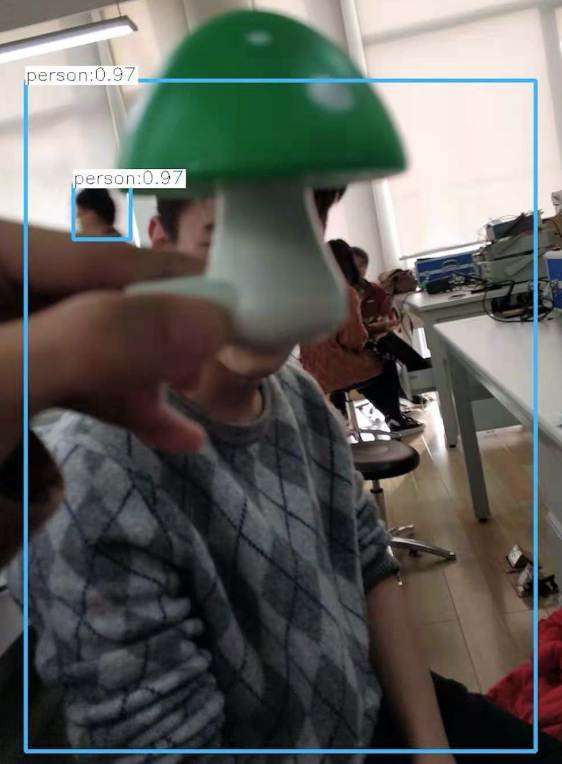
\includegraphics[width=\linewidth]{figures/det.png}
%     \end{minipage}\label{fig:det}
%     }
%     %
%     \centering
%     \subfigure[语义分割]{
%     \begin{minipage}[t]{0.28\linewidth}
%     \centering
%     
\includegraphics[width=\linewidth]{figures/seg.png}
%     \end{minipage}\label{fig:seg}
%     }
%     %
%     \centering
%     \subfigure[姿态识别]{
%     \begin{minipage}[t]{0.4\linewidth}
%     \centering
%     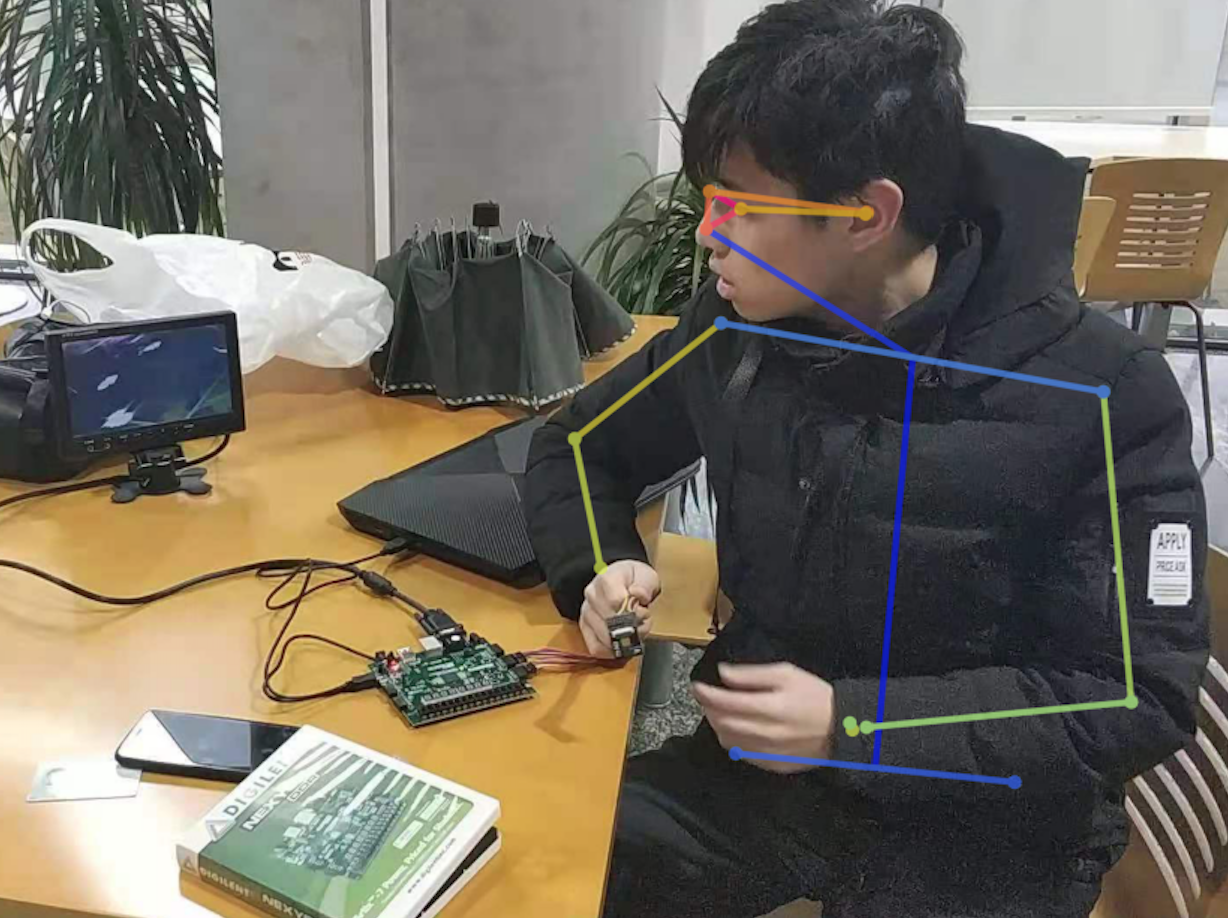
\includegraphics[width=\linewidth]{figures/pose.png}
%     \end{minipage}\label{fig:pose}
%     }
%     %
%     \caption{常见视频分析应用图解(图片提供者为中中同学)}\label{fig:cvexample}
%     \centering
% \end{figure}